\chapter{Introduction to Digital Forensics}
\section{What does forensics mean?}
    \begin{itemize}
        \item \textbf{Forensics} is the application of scientific analysis to reconstruct evidence.
        \item \textbf{Digital Forensics} is one of the disciplines of forensics, is the application of scientific analysis methods to digital data, computer systems, and network data to reconstruct evidence.
    \end{itemize}
    Forensics is strongly related with laws: different jurisdiction means different procedures.
\section{The Daubert standard (USA)}
    Generally speaking, we can have two sources of evidence:
    \begin{itemize}
        \item physical evidence
        \item eyewitness testimony
    \end{itemize}
    To provide physical evidence, an expert is allowed to give an opinion in court because of the fact that he is an expert, and the use of scientific methods is the reason why he is listened to.\\
    How do we define what an expert is?
    \subsection{The Daubert Standard}
        We define as expert witness someone who has witness because of its own experience.\\
        The Daubert standard define an expert witness as follows:\\
        A witness who is qualified as an expert by knowledge, skill, experience, training, or education may testify in the form of an opinion or otherwise if:
        \begin{itemize}
            \item The expert's scientific, technical, or other specialized knowledge will help the trier of fact\footnote{the judge} to understand the evidence or to determine a fact in issue;
            \item The testimony is based on sufficient facts or data;
            \item The testimony is the product of reliable principles and methods; and
            \item The expert has reliably applied the principles and methods to the facts of the case.
        \end{itemize}
    Reliable principles and methods means that they are scientifically found. You need an expert to use scientific method to establish those facts:
    \subsection{What is scientific? (Italy)}
        \begin{itemize}
            \item Galileo: scientific means repeatable, you actually make an experiment to demonstrate that something can happen
            \item Popper: scientific means falsifiable, if you're able to create, at least in your mind, an example which proves the opposite of a statement, then the statement is scientific.
            \begin{itemize}
                \item Example: \textit{Stefano is a kind person} is not a scientific statement, because it is not falsifiable.
            \end{itemize}
        \end{itemize}
        Some of the questions are not falsifiable, hence not scientific. An example is a criminal which keeps images of kids on his own computer. Did he do it willingly or not? This is not falsifiable.\\
        What is possible to do is to look at the folder to see if it was opened multiple times, look at the file to see if it was in the browser's cache or in a specific folder on the criminal's computer.
    \subsection{Daubert Test for scientific}
    Factors to consider (USA) to establish if something is scientific or not:
    \begin{itemize}
        \item Whether the theory or technique employed by the expert is generally accepted in the scientific community
        \item Whether it has been subjected to peer review and publication
        \item Whether it can be and has been tested
        \item Whether the known or potential rate of error is acceptable; and
        \item Whether the research was conducted independent of the particular litigation or dependent on an intention to provide the proposed testimony.
    \end{itemize}
\section{Example of forensic engagements}
    We do forensics for different situations in different contexts
    \begin{figure}[ht!]
        \centering
        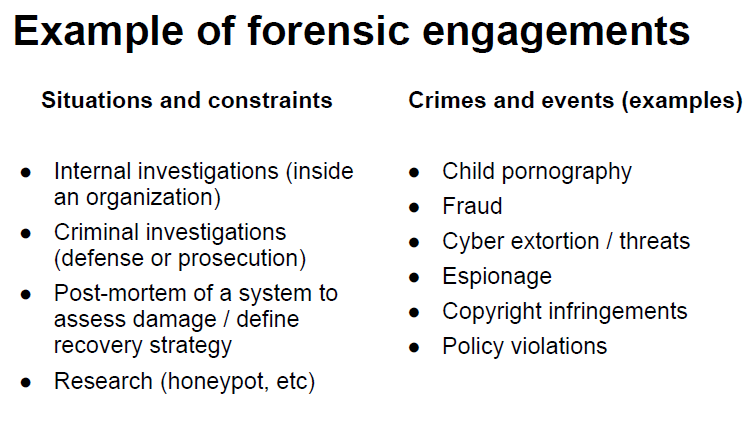
\includegraphics[width=0.5\linewidth]{lecture_3/forensics.png}
    \end{figure}
    \\Depending on which part of the lawsuit you're working for: \textit{("prosecutor", "judge", "lawyer")}, the things that you can do are different.\\
    The procedures has always to be contextualized in what are the purposes and which constraints the purpose has.          

    %%%%
    If we're investigating in the 1st two out of the situations and constraint things:
        singlemost investigated prosecuted type of crime is %banned from github
        the second one is Fraud

        Reality: the reason why the 1st one of examples is prosecuted is because it is the easiest one to prosecute
        this has an effect: if you do forensics as a job, you'll see those images, 

    Fraud is the other INVESTIGATED crime: prosecuting fraud is difficult. Large amount of them happens spread trough the network and criminals live in countries with bad laws

    if you denounce you do it to get your money back but they never prosecuted or just investigated for this reason

    Cyber extortion: the kind of it that is widely prosecuted is extortion of personal things like i stole your data or information and want you to pay me
        extortion happen in family, work related, interpersonal relationship, revenge corn cases.

    fundamentally cybercrimes.

    Also a lot of non-cyber crimes with digital components:
        in case of murder check the digital devices to search for traces
        tracking or geolocalization of mobile devices 
        traces on gps navigators

        digital components can be fundamental.

    Something which is borderline, only subject of a lawsuit and not crimes:
        espionage: stealing from old company to new one --> sometimes criminal investigation, very often lawsuit for damages + termination 

\section{Phases of an investigation (Pollitt)}
    \begin{itemize}
        \item Source acquisition: how we preserve digital evidence
        \item Evidence identification: how we analyze digital evidence 
        \item Evaluation: how we take evidence and pack with the specific case
        \item Presentation: how we put togheter all of this in a court
    \end{itemize}